\documentclass[10pt, letterpaper]{l3doc}

\hypersetup{urlcolor = teal, filecolor = violet}
\hologoFontSetup{general = \sffamily}
\usepackage[mono = false]{libertine}
\usepackage{geometry,framed,xeCJKfntef,enumitem}
\setlength{\oddsidemargin}{63pt}\setlength{\evensidemargin}{63pt}
\FrameSep = 0pt 
\usepackage[os = mac]{menukeys}
\AddToHook{env/function/before}{\vspace{-.3\baselineskip}}
\AddToHook{env/syntax/after}{\vspace{-.2\baselineskip}}
\usepackage{datetime}
\yyyymmdddate
\usepackage[fontset = none, scheme = plain]{ctex}
\linespread{1.3}
\setCJKmainfont[AutoFakeSlant]{Songti SC}
\setCJKsansfont[BoldFont = Hei, AutoFakeSlant]{Heiti SC}
\setCJKmonofont[AutoFakeSlant]{LXGW WenKai}
\renewcommand{\emph}[1]{\CJKsout*[thickness=2.5ex, format=\color{blue!15}]{#1}}

\title{\bfseries The \textsc{\cls{HduThesis}} Class\\
\hologo{LaTeX} Thesis Template for Hangzhou Dianzi University}
\author
{
  Mingyu Xia \texttt{<\href{mailto:xiamyphys@gmail.com}{xiamyphys@hdu.edu.cn}>}
  \footnote{
    School of Sciences, Physics Department, Graduate in 06/2025 (expected)
  }
}
\date{v0.1.0\footnote{\url{https://github.com/xiamyphys/litetable}} ~(\today)}

\begin{document}

\newgeometry{margin = 1in}
\begin{titlepage}
  \maketitle
  \begin{center}
    \tikz
    {
      \node [opacity = .8] 
      {
\includegraphics[width = .2\paperwidth]{./figures/hdumotto.pdf}};
      \node [opacity = .3]
      {
\includegraphics[width = .3\paperwidth]{./figures/hdulogo.pdf}};
    }
  \end{center}
  \begin{abstract}
    \textsc{\pkg{HDUThesis}} 是杭州电子科技大学毕业论文 \hologo{LaTeX}模板,
    支持学士论文排版. 后续会扩展到硕士、博士论文.
    \vspace*{1em}
    \begin{center}
      \footnotesize\bfseries User Agreement
    \end{center}
    \begin{enumerate}[leftmargin = 2.5ex]
      \item 本模板通过 LPPL 1.3c 协议开放源代码,您可以随意使用编译出的 PDF 文件.
      \item 截止本文档编译时,杭州电子科技大学教务处只提供Word模板
      \footnote
      {
        \url{https://jwc.hdu.edu.cn/2022/0428/c4528a153813/page.htm}
      }. 作者不对使用本模板产生的格式审查问题负责.
      \emph{如果您所在的学院要求提交 \cmd{.docx} 格式的论文稿件,请勿执意使用本模板,
      避免因格式转换带来不必要的麻烦.} 欢迎前往 GitHub 提交反馈意见,为推动学校认证与规范化
      \textsc{\cls{HduThesis}} 贡献力量.
    \end{enumerate}
  \end{abstract}
  \thispagestyle{empty}
\end{titlepage}

\restoregeometry

\section{Generate the Cover}

\begin{function}{\DocInfo}
  \begin{syntax}
    \cs{DocInfo}\marg{keyvals}
  \end{syntax}

  此命令接收键值,用于设置文档信息. 键 \keys{\cmdmac~title} 用于设置论文标题,
  键 \keys{\cmdmac~school} 用于设置学院,键 \keys{\cmdmac~major} 用于设置专业,
  键 \keys{\cmdmac~class} 用于设置班级,键 \keys{\cmdmac~stdntid} 用于设置学号,
  键 \keys{\cmdmac~author} 用于设置作者,键 \keys{\cmdmac~supervisor} 用于设置导师.

  \begin{framed}
    \begin{verbatim}
    \documentclass{hduthesis}
    \DocInfo
    {
      title      = XXXXXX ,  school     = 理学院,  major      = ,  class      = ,
      stdntid    = ,         author     = ,        supervisor = ,
    }
    \begin{document}  \maketitle    ...    \end{document}
    \end{verbatim}
  \end{framed}

  \begin{center}
    \fbox{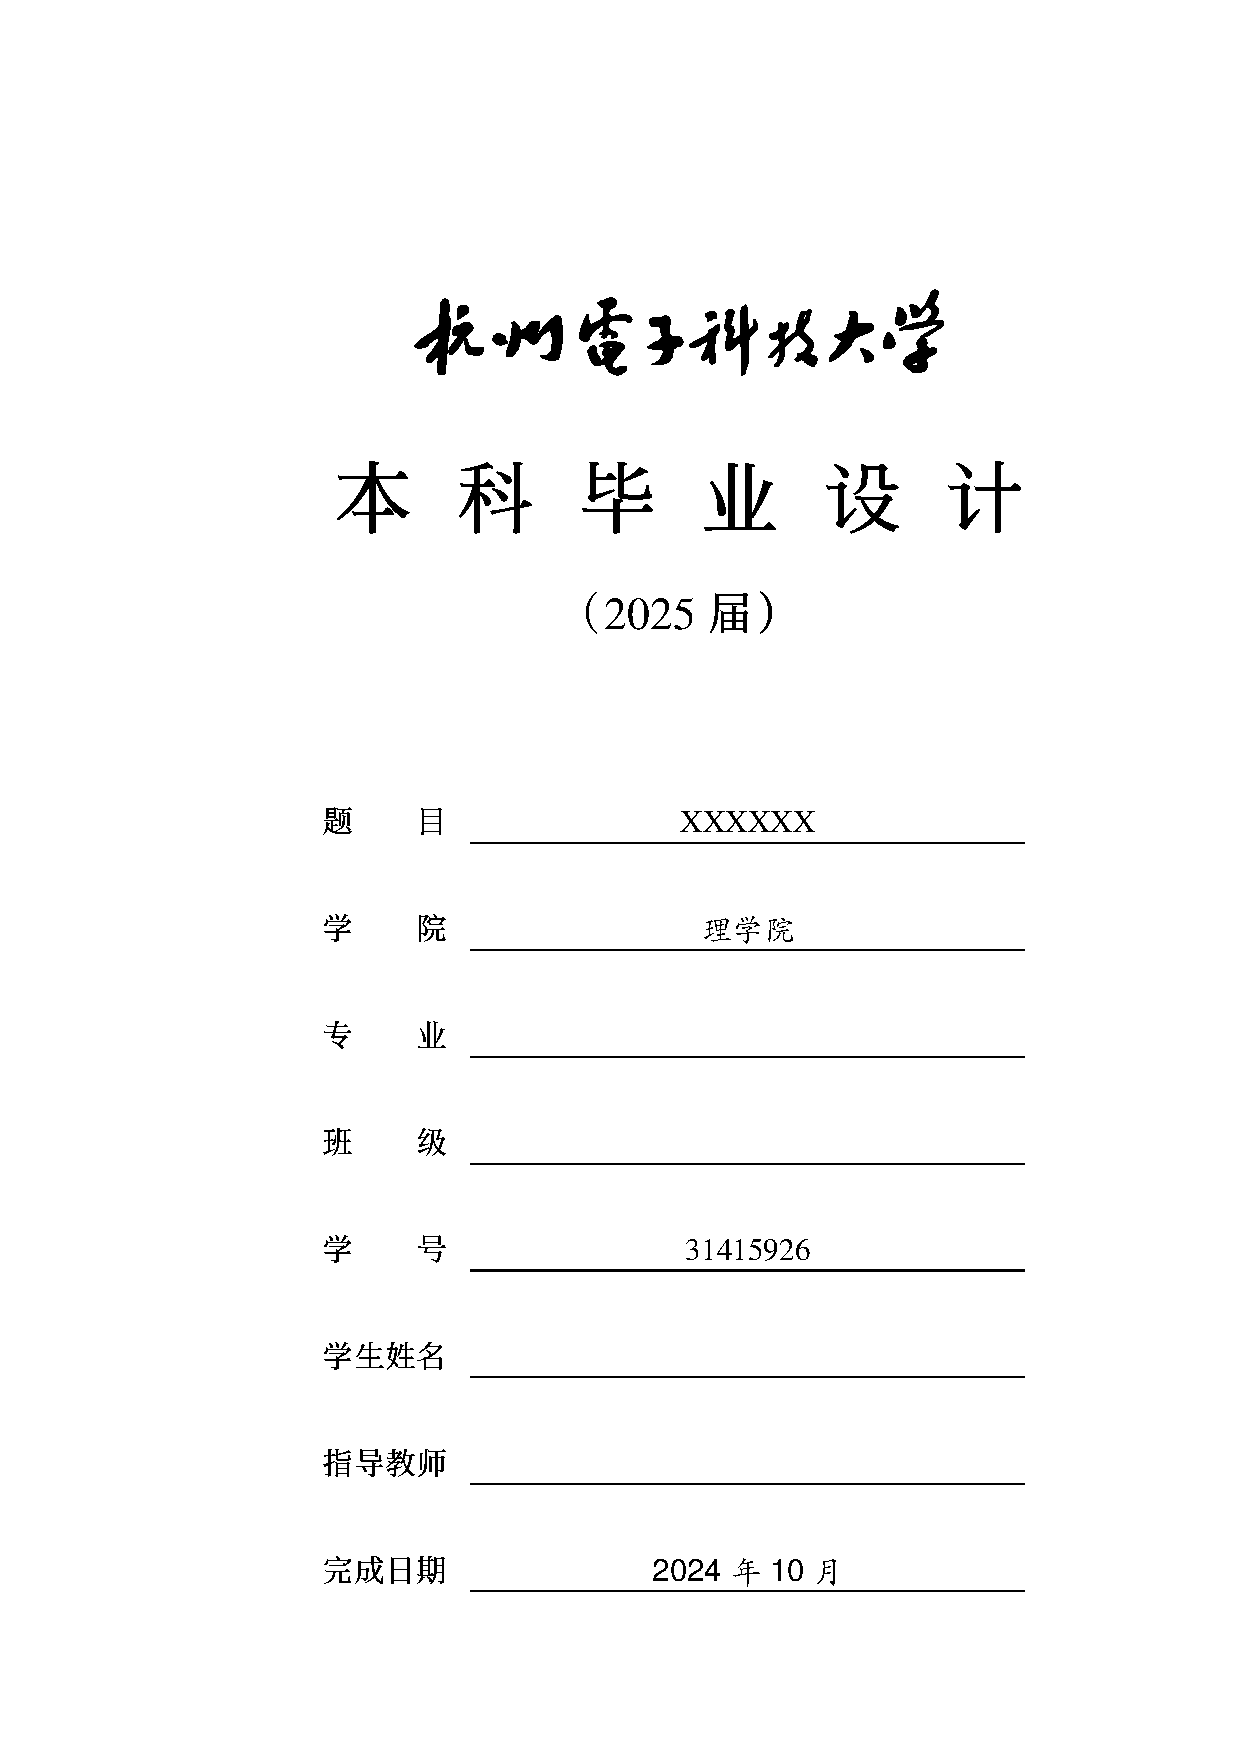
\includegraphics[page = 1, width = .432\linewidth]{hduthesis-demo}}
    \hfill
    \fbox{\includegraphics[page = 2, width = .432\linewidth]{hduthesis-demo}}
  \end{center}

  命令 \cs{DocInfo} 需在导言区中执行. 通过此命令完成文档信息输入后,
  在 \verb|\begin{document}| 后执行命令 \cs{maketitle} 会调用所设置的键值并自动生成\emph{论文封面}和\emph{诚信承诺书}.
\end{function}

论文完成日期和学生毕业年份会根据当前系统时间自动生成.
如果当前月份在8月及以前,毕业年份会显示当前年;如果当前月份在9月及以后,毕业年份会显示次年. 
如果执意要更改毕业年份,则需在导言区中命令 \cs{DocInfo} 后输入

\begin{framed}
  \begin{verbatim}
    \ExplSyntaxOn
      \int_set:Nn \l__hduthesis_grade_int {<Graduate Year>}
    \ExplSyntaxOff
  \end{verbatim}
\end{framed}

\section{Enter Abstract in EN / CN}

\begin{function}{abstract (env.),\keywords}
  \begin{syntax}
    \cs{begin}\{abstract\}[en]  ...\cs{keywords}\marg{keywords list}  \cs{end}\{abstract\}
    \cs{begin}\{abstract\}[cn]  ...\cs{keywords}\marg{关键词列表}      \cs{end}\{abstract\}
  \end{syntax}

  环境 \env{abstract} 用于生成摘要,其可选参数可设置语言格式.
  命令 \cs{keywords} 需在 \env{abstract} 环境内执行,
  其会根据 \env{abstract} 环境所选择的语言,自动生成英文 / 中文格式的关键词.
  
  通过命令 \cs{keywords} 以半角逗号 (,) 为分隔输入关键词列表,
  输出时会根据所处 \env{abstract} 环境选择的语言不同,自动以半 / 全角分号分隔.
  
  \begin{center}
    \fbox{\includegraphics[page = 3, width = .432\linewidth]{hduthesis-demo}}
    \hfill
    \fbox{\includegraphics[page = 4, width = .432\linewidth]{hduthesis-demo}}
  \end{center}
\end{function}

\section{Input Text}

\textsc{\cls{HduThesis}} 的 {chapter}、\cs{section}、\cs{subsection}、\cs{enumerate} 等段落级次均已按``\href{https://jwc.hdu.edu.cn/2022/0428/c4528a153813/page.htm}{杭电理工类毕业论文写作规范}''定制,可直接使用.

\begin{center}
  \fbox{\includegraphics[page = 5, width = .3\linewidth]{hduthesis-demo}}
  \hfill
  \fbox{\includegraphics[page = 11, width = .3\linewidth]{hduthesis-demo}}
  \hfill
  \fbox{\includegraphics[page = 12, width = .3\linewidth]{hduthesis-demo}}
\end{center}

同时,模板额外预制了如下宏包

\begin{table}[htbp]
  \centering
  \begin{tabular}{*{6}{p{.13\linewidth}}}
    \toprule
    \pkg{amsmath}    & \pkg{amssymb}   & \pkg{bm} &
    \pkg{booktabs}   & \pkg{cancel}    & \pkg{cleveref}\\
    \midrule
    \pkg{derivative} & \pkg{extarrows} & \pkg{fixdif} &
    \pkg{mathtools}  & \pkg{multicol}  & \pkg{physics2}\\
    \bottomrule
  \end{tabular}
\end{table}

如需插入参考文献,在导言区使用命令 \cs{addbibsource}\marg{.bib file name}导入
\file{.bib} 文件,并在文章末尾输入 \cs{printbiblography} 即可.
文档已将参考文献格式设置为 \cmd{gb7714-2015}.

\appendix\clearpage

\section{The Code}

\textsc{\cls{HduThesis}} 文档类采用模块化设计,根文件 \file{hduthesis.cls} 中
\cs{key_define:} 用于声明文档信息的键,并调用其他模块.

\begin{enumerate}
  \item 字体配置模块存放于 \file{hduthesis-font-module.code.tex} 中.
  \item 封面信息模块存放于 \file{hduthesis-cover-module.code.tex} 中,
  分别使用 \cs{l_spread_box} 和 \cs{l_center_box} 实现分散对齐和居中划线.
  \item 中英摘要模块存放于 \file{hduthesis-matter-module.code.tex} 中,
  使用 \cs{str_if_eq:nnT} 对摘要语言进行判断.
  \item 章节段落模块存放于 \file{hduthesis-layout-module.code.tex} 中,
  参照\emph{标准文档类}说明文档 (\cmd{texdoc classes}),对相应的宏进行重新定义.
  后期维护者可考虑使用 \pkg{titlesec} 包.
\end{enumerate}

\begin{framed}
  \begin{verbatim}
    % 预留学号接口,用于后续判断学位.
    \cs_new_protected_nopar:Npn \int_if_exist_use:N #1
      {
        \int_compare:nNnT #1 > 0
          {
            \int_use:N #1
          }
      }
    \keys_define:nn { hduthesis / docinfo }% 声明相应键
      {
      title.tl_set:N = \l__docinfo_title_tl,
      school.tl_set:N = \l__docinfo_school_tl,
      major.tl_set:N = \l__docinfo_major_tl,
      class.tl_set:N = \l__docinfo_class_tl,
      stdntid.int_set:N = \l__docinfo_stdntid_int,
      author.tl_set:N = \l__docinfo_author_tl,
      supervisor.tl_set:N = \l__docinfo_supervisor_tl,
    }
    \NewDocumentCommand \DocInfo { m }
      {
        \keys_set:nn { hduthesis / docinfo } { #1 }
      }
  \end{verbatim}    
\end{framed}

\end{document}
